\documentclass[10pt]{article}
\usepackage[a4paper,margin=5mm,landscape]{geometry}
\usepackage{blindtext}

\usepackage{multicol}
\usepackage{enumitem}
\usepackage[dvipsnames]{xcolor}
\usepackage{graphicx}



\usepackage[condensed,math]{iwona}

\usepackage[sfdefault,condensed]{roboto}  %% Option 'sfdefault' only if the base font of the document is to be sans serif
\usepackage[T1]{fontenc}


% Marca d'agua
%\usepackage{draftwatermark}
%\SetWatermarkText{Draft}
%\SetWatermarkScale{5}

\setlength{\columnseprule}{.5pt}
\linespread{.95}

\usepackage{titlesec}
\titlespacing{\subsection}{0pc}{3.pt}{1.pt}
\titlespacing{\subsubsection}{0pc}{1.5pt}{1.pt}

\definecolor{mygray}{RGB}{250, 250, 250}
\pagecolor{mygray}

\usepackage{float}

\setlength{\textfloatsep}{1pt}
\setlength{\floatsep}{1pt}
\setlength{\intextsep}{1pt}

\begin{document}
\noindent
{\Large{\textbf{\emph{C++ Standard Template Library (STL) Quick Reference}}, {\small version 1.0}}	
}

\noindent
{\small  Roberto D. Algarte (2024)}

\scriptsize
\begin{multicols*}{5}

{\color{Blue}
\subsection*{NOTATION}	

\begin{itemize}[leftmargin=*,topsep=0.25pt]
  \setlength\itemsep{-1.8pt}
	\item \textbf{priority\_queue} @ $<$queue$>$: class ``pri\-ori\-ty\_que\-ue'' that belongs to library ``queue'';
	\item \emph{\textbf{setbase}} @ $<$iomanip$>$: standalone function ``setbase'' that belongs to library ``iomanip'';
	\item stream.\emph{\textbf{good}} @ $<$iostream$>$: member function ``good'' of an object from class ``stream'' that belongs to ``iostream''; REVER
\end{itemize}

}

{\color{Blue}
\subsection*{CONTAINERS}	
\noindent
Aggregates of elements that provide element insertion, removal and access.

\subsubsection*{\textsc{Theory} - \emph{Time Complexity}} 
\begin{figure}[H]
\begin{center}
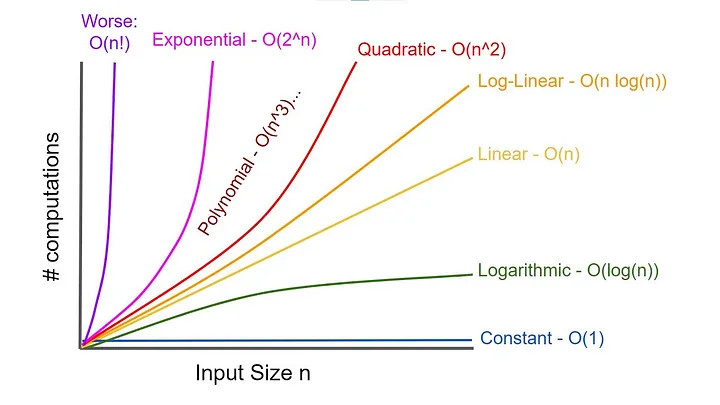
\includegraphics[scale=.21]{complexity.jpg}	
\end{center}
\end{figure}

\subsubsection*{\textsc{Theory} - \emph{Linear Aggregates}} 

\begin{itemize}[leftmargin=*,topsep=0.25pt]
  \setlength\itemsep{-1.8pt}
	\item \emph{Array}: static or dynamic structure whose elements have defined positions and are stored in contiguous memory. Insertion and removal of elements may imply repositioning of other elements or repositioning of the entire structure; 
	\item \emph{Linked list}: dynamic structure whose elements may not be stored contiguously. A node (list element) is composed by a value and one or two references to adjacent nodes. Nodes of a \emph{doubly-linked} list have two references, and of a \emph{singly-linked}, one reference. Insertion and removal don't imply repositioning of other elements;
	\item \emph{Stack}: LIFO dynamic structure with one end, in which insertion, deletion and access are performed;
	\item \emph{Queue}: FIFO dynamic structure with two ends, one for insertion and another for removal; access can be performed on both. In a \emph{double-ended} queue, both ends allow insertion and removal;  
\end{itemize}

\subsubsection*{\textsc{Sequence Containers}} 
\noindent
Containers whose elements can be accessed sequentially and are stored contiguously in memory.

\begin{itemize}[leftmargin=*,topsep=0.25pt]
  \setlength\itemsep{-1.8pt}
	\item \textbf{array} @ $<$array$>$: wrapper for C static arrays;
	\item \textbf{vector} @ $<$vector$>$: implementation of a dynamic array. Insertion and removal are $O(1)$ at the end, $O(n)$ elsewhere; access is $O(1)$;
	\item \textbf{dequeue} @ $<$dequeue$>$: implementation of a double-ended queue. Insertion, removal and access are $O(1)$;
	\item \textbf{forward\_list} @ $<$forward\_list$>$: implementation of a singly-linked list. Insertion and removal are $O(1)$; access is $O(n)$. Provided by $<$forward\_list$>$;  
	\item \textbf{list} @ $<$list$>$: implementation of a doubly-linked list. Insertion and removal are $O(1)$; access is $O(n)$;
\end{itemize}

\subsubsection*{\textsc{Sequence Container Adapters}} 
\noindent
Wrappers created around dequeue to provide other types of aggregates.

\begin{itemize}[leftmargin=*,topsep=0.25pt]
  \setlength\itemsep{-1.8pt}
	\item \textbf{stack} @ $<$stack$>$: implementation of a stack;
	\item \textbf{queue} @ $<$queue$>$: implementation of a simple queue;
	\item \textbf{priority\_queue} @ $<$queue$>$: implementation of a queue in which the front element must observe a priority condition (the largest, by default). Insertion and removal are $O(log(n))$;
\end{itemize}
\noindent

\subsubsection*{\textsc{Associative Containers}} 
\noindent
Containers constituted by (non)primary key sorted elements or pair of (non)primary key-value sorted elements that are  inserted, removed and accessed in $O(log(n))$ time complexity for the worst case.

\begin{itemize}[leftmargin=*,topsep=0.25pt]
  \setlength\itemsep{-1.8pt}
	\item \textbf{set} @ $<$set$>$: constituted by primary key elements;
	\item \textbf{map} @ $<$map$>$: constituted by primary key-value elements;
	\item \textbf{multiset} @ $<$set$>$: constituted by non primary key elements;
	\item \textbf{multimap} @ $<$map$>$: constituted by non primary key-value elements;  
\end{itemize}
\noindent
Each one of these types has its \textbf{unordered\_*} counterpart, whose elements are inserted or removed in $O(1)$, and accessed in $O(n)$ for the worst case. 


}

\par\noindent\rule{155pt}{0.4pt}

{\color{Blue}
\subsection*{I/O STREAMS}	
\noindent
Streams enable flow of data to be written (output) or to be read (input). Output streams can be buffered or not.
The \emph{extractor operator} $<<$ when applied to input streams performs formatted input while the \emph{insertion operator} $>>$ applied to output streams performs formatted output. 

\subsubsection*{\textsc{Console Streams}} 
\begin{itemize}[leftmargin=*,topsep=0.25pt]
  \setlength\itemsep{-1.8pt}
	\item \textbf{cin} @ $<$iostream$>$: wrapper around the standard C stream stdin, which reads data from the console;
	\item \textbf{cout} @ $<$iostream$>$: wrapper around the standard C stream stdout, which writes data to the console and is buffered;
	\item \textbf{cerr} @ $<$iostream$>$: wrapper around the standard C stream stderr, which writes data to the console;
\end{itemize}

\subsubsection*{\textsc{String Streams}}
\noindent
Streams that enable flow of outputted or inputted strings.

\begin{itemize}[leftmargin=*,topsep=0.25pt]
  \setlength\itemsep{-1.8pt}
	\item \textbf{basic\_istringstream} @ $<$sstream$>$: provides high level string input formatting;
	\item \textbf{basic\_ostringstream} @ $<$sstream$>$: provides high level string output formatting;
	\item \textbf{basic\_stringstream} @ $<$sstream$>$: provides high level string input/output formatting;
\end{itemize}


\subsubsection*{\textsc{File Streams}} 
\noindent
Streams that enable flow of outputted or inputted data to or from files.

\begin{itemize}[leftmargin=*,topsep=0.25pt]
  \setlength\itemsep{-1.8pt}
	\item \textbf{basic\_ifstream} @ $<$fstream$>$: provides high level file input formatting;
	\item \textbf{basic\_ofstream} @ $<$fstream$>$: provides high level file output formatting;
	\item \textbf{basic\_fstream} @ $<$fstream$>$: provides high level file input/output formatting;
\end{itemize}

\subsubsection*{\textsc{Aliases}} 
\begin{itemize}[leftmargin=*,topsep=0.25pt]
  \setlength\itemsep{-1.8pt}
	\item \textbf{istringstream} $=$ \textbf{basic\_istringstream}<char>;
	\item \textbf{ostringstream} $=$ \textbf{ba\-sic\_o\-string\-stream}\-<char>;
	\item \textbf{stringstream} $=$ \textbf{basic\_stringstream}<char>;
	\item \textbf{ifstream} $=$ \textbf{basic\_ifstream}<char>;
	\item \textbf{ofstream} $=$ \textbf{basic\_ofstream}<char>;
	\item \textbf{fstream} $=$ \textbf{basic\_fstream}<char>;
\end{itemize}


\subsubsection*{\textsc{Manipulators and Formatters}} 
\begin{itemize}[leftmargin=*,topsep=0.25pt]
  \setlength\itemsep{-1.8pt}
	\item \textbf{boolalpha} @ $<$ios$>$: sets text values for booleans;
	\item \textbf{showbase} @ $<$ios$>$: enables base prefix in numbers;
	\item \textbf{showpoint} @ $<$ios$>$: enables decimal point in numbers;
	\item \textbf{showpos} @ $<$ios$>$: pre-print a $+$ in nonnegative numbers;
	\item \textbf{skipws} @ $<$ios$>$: skips white spaces;
	\item \textbf{unitbuf} @ $<$ios$>$: sets buffer flushing for every output operation;
	\item \textbf{hex} @ $<$ios$>$: outputs in base 16;
	\item \textbf{oct} @ $<$ios$>$: outputs in base 8;
	\item \textbf{fixed} @ $<$ios$>$: outputs floats in fixed width;
	\item \textbf{scientific} @ $<$ios$>$: outputs floats in scientific notation;
	\item \textbf{hexfloat} @ $<$ios$>$: outputs floats in hex notation;
	\item \textbf{defaultfloat} @ $<$ios$>$: outputs floats as default;
	\item \emph{\textbf{setbase}} @ $<$iomanip$>$: sets the output base;
	\item \emph{\textbf{setfill}} @ $<$iomanip$>$:sets a fill character instead of white space;
	\item \emph{\textbf{setprecision}} @ $<$iomanip$>$: sets the precision of floats;
	\item \emph{\textbf{setw}} @ $<$iomanip$>$: sets the output width for the text;
	\item \emph{\textbf{get\_money}} @ $<$iomanip$>$: parse value as currency;
	\item \emph{\textbf{put\_money}} @ $<$iomanip$>$: sets values to currency;
	\item \emph{\textbf{get\_time}} @ $<$iomanip$>$: parses value as a datetime;
	\item \emph{\textbf{put\_time}} @ $<$iomanip$>$: outputs a \textbf{std:tm} object with specified format;
	\item \emph{\textbf{quoted}} @ $<$iomanip$>$: correctly reads and writes strings with quotes;
	\item \emph{\textbf{flush}} @ $<$ostreamp$>$: flushes the stream buffer;
	\item \emph{\textbf{endl}} @ $<$ostream$>$: inserts a line break and flushes the buffer;
	\item \emph{\textbf{ends}} @ $<$iomanip$>$: inserts a null character;
	\item \emph{\textbf{getline}} @ $<$string$>$: reads a line from input stream setting the reading pointer to the new line. By default, lines are separated by line breaks;
\end{itemize}

\subsubsection*{\textsc{States}} 
\begin{itemize}[leftmargin=*,topsep=0.25pt]
  \setlength\itemsep{-1.8pt}
	\item stream.\emph{\textbf{good}} @ $<$iostream$>$: stream is fine an can be read or written to;
	\item stream.\emph{\textbf{bad}} @ $<$iostream$>$: stream is in a non recoverable error state;
	\item stream.\emph{\textbf{eof}} @ $<$iostream$>$: reading pointer arrived at the end of file;
	\item stream.\emph{\textbf{fail}} @ $<$iostream$>$: stream is in a recoverable error state;
	\item stream.\emph{\textbf{clear}} @ $<$iostream$>$: refresh the state of the stream;
\end{itemize}


}

\par\noindent\rule{155pt}{0.4pt}

{\color{Blue}
\subsection*{ITERATORS}	
\noindent
Pointer-like types created to implement the iterator pattern in STL. The iterator pattern states that aggregate structures and element-accessing functions should be decoupled.

\subsubsection*{\textsc{Iteratable Aggregates}} 
\noindent
All types of STL containers, C arrays, input and output streams.

\subsubsection*{\textsc{Concepts}} 
\begin{itemize}[leftmargin=*,topsep=0.25pt]
  \setlength\itemsep{-1.8pt}
	\item \textbf{output\_iterator} @ $<$iterator$>$: a type that can be both pre- and post-incremented, related to a given structure to which values can be written (e.g. output streams);
	\item \textbf{ostream\_iterator} @ $<$iterator$>$: a specific type of out\-put\_i\-te\-ra\-tor that writes to an output stream;
	\item \textbf{input\_iterator} @ $<$iterator$>$: a type that can be both pre- and post-incremented, related to a given structures whose values can be read (e.g. input streams);
	\item \textbf{istream\_iterator} @ $<$iterator$>$: a specific type of in\-put\_i\-te\-ra\-tor that reads from an input stream;
	\item \textbf{forward\_iterator} @ $<$iterator$>$: an input\_iterator that has equality comparison and multi-pass, which means that it can traverse multiple times the elements of an aggregate (e.g. containers); 
	\item \textbf{bidirectional\_iterator} @ $<$iterator$>$: a forward\_iterator able to traverse backwards; 
	\item \textbf{random\_access\_iterator} @ $<$iterator$>$: a bidirectional\_iterator that supports subscripting with $O(1)$ time access to elements; 
	\item \textbf{contiguous\_iterator} @ $<$iterator$>$: a specific ran\-dom\_ac\-cess\_i\-te\-ra\-tor that traverses elements stored contiguously in memory (e.g. vector). 
\end{itemize}

\subsubsection*{\textsc{Range Functions}} 
\begin{itemize}[leftmargin=*,topsep=0.25pt]
  \setlength\itemsep{-1.8pt}
	\item  \emph{\textbf{begin}} @ $<$iterator$>$: returns the first element read-write iterator. The function \emph{\textbf{cbegin}} returns the read-only version;
	\item  \emph{\textbf{end}} @ $<$iterator$>$: returns the one-past-the-last element read-write iterator. The function \emph{\textbf{cend}} returns the read-only version;
	\item  \emph{\textbf{rbegin}} @ $<$iterator$>$: returns the first element read-write reverse iterator. The function \emph{\textbf{crbegin}} returns the read-only version;
	\item  \emph{\textbf{rend}} @ $<$iterator$>$: returns the one-past-the-last element read-write reverse iterator. The function \emph{\textbf{crend}} returns the read-only version;
\end{itemize}

\subsubsection*{\textsc{Adapters}} 
\noindent
Iterator wrappers created to encapsulate some important iterator-related functionalities. 
\begin{itemize}[leftmargin=*,topsep=0.25pt]
  \setlength\itemsep{-1.8pt}
	\item \textbf{reverse\_iterator} @ $<$iterator$>$: performs reverse order traversal. This adapter can be created by the helper function \emph{\textbf{make\_reverse\_iterator}};
	\item \textbf{move\_iterator} @ $<$iterator$>$: performs move of elements from one aggregate to another. This adapter can be created by the helper function \emph{\textbf{make\_move\_iterator}};
	\item \textbf{insert\_iterator} @ $<$iterator$>$: performs insertion of element at a specified position. This adapter can be created by the helper function \emph{\textbf{inserter}};
	\item \textbf{back\_insert\_iterator} @ $<$iterator$>$: performs back insertion of elements. This adapter can be created by the helper function \emph{\textbf{back\_inserter}};
	\item \textbf{front\_insert\_iterator} @ $<$iterator$>$: performs front insertion of elements. This adapter can be created by the helper function \emph{\textbf{front\_inserter}};
\end{itemize}

\subsubsection*{\textsc{Operations}} 
\begin{itemize}[leftmargin=*,topsep=0.25pt]
  \setlength\itemsep{-1.8pt}
	\item  \emph{\textbf{distance}} @ $<$iterator$>$: returns the number of elements between two iterators in which the first is included and last excluded;
	\item  \emph{\textbf{advance}} @ $<$iterator$>$: advances an iterator by a given distance;
	\item  \emph{\textbf{next}} @ $<$iterator$>$: increments an iterator returning it;
	\item  \emph{\textbf{prev}} @ $<$iterator$>$: decrements an iterator returning it;
	\item  \emph{\textbf{empty}} @ $<$iterator$>$: checks whether the given range empty;
	\item  \emph{\textbf{data}} @ $<$iterator$>$: returns the pointer the given sequence container;
\end{itemize}

\par\noindent\rule{155pt}{0.4pt}

{\color{Blue}
\subsection*{ALGORITHMS}	
\noindent
Collection of libraries providing a variety of functionalities like searching, counting, sorting, partitioning and transforming, applied to a range of elements.

\subsubsection*{\textsc{Sorting Functions}} 
\begin{itemize}[leftmargin=*,topsep=0.25pt]
  \setlength\itemsep{-1.8pt}
	\item  \emph{\textbf{sort}} @ $<$algorithm$>$: sorts a range in ascending order;
	\item  \emph{\textbf{is\_sorted}} @ $<$algorithm$>$: checks if the elements are non-descending ordered;
	\item  \emph{\textbf{is\_sorted\_until}} @ $<$algorithm$>$: finds the largest sub-range inside a range whose elements are non-descending ordered;
	\item  \emph{\textbf{partial\_sort}} @ $<$algorithm$>$: sorts a range in ascending order from begin until a specified position;
	\item  \emph{\textbf{partial\_sort\_copy}} @ $<$algorithm$>$: copies an ascending sorts from begin until a specified position of a range to another range;
	\item  \emph{\textbf{stable\_sort}} @ $<$algorithm$>$: sorts a range in ascending order such that the original order of equally indexed elements of multi-associative containers is preserved;
	\item  \emph{\textbf{nth\_element}} @ $<$algorithm$>$: rearranges the elements in such a way that the value at the position n corresponds to the n-th element of the sorted range;
\end{itemize}

\subsubsection*{\textsc{Main Modifying Functions}} 
\begin{itemize}[leftmargin=*,topsep=0.25pt]
  \setlength\itemsep{-1.8pt}
	\item  \emph{\textbf{copy}} @ $<$algorithm$>$: copies a range, from beginning to end, to another range;
	\item  \emph{\textbf{copy\_if}} @ $<$algorithm$>$: copies a range, from beginning to end, to another range that obey a predicate;
	\item  \emph{\textbf{copy\_n}} @ $<$algorithm$>$: copies n elements of a range, from beginning to end, to another range;
	\item  \emph{\textbf{copy\_backward}} @ $<$algorithm$>$: copies a range, from end to beginning, to another range;
	\item  \emph{\textbf{reverse\_copy}} @ $<$algorithm$>$: copies a range of size n, from end to beginning, to another range of size n;
	\item  \emph{\textbf{move}} @ $<$algorithm$>$: moves the elements of a range, from beginning to end, to another range. Afterwards, the elements of the source range are left in undefined state;
	\item  \emph{\textbf{move\_backward}} @ $<$algorithm$>$: moves the elements of a range, from end to beginning, to another range. Afterwards, the elements of the source range are left in undefined state;
	\item  \emph{\textbf{swap}} @ $<$algorithm$>$: moves the values of two variables to one another;
	\item  \emph{\textbf{swap\_ranges}} @ $<$algorithm$>$: swaps every element of a n-distance range with another n-distance range;
	\item  \emph{\textbf{iter\_swap}} @ $<$algorithm$>$: swaps values pointed by two iterators;
		\item  \emph{\textbf{remove}} @ $<$algorithm$>$: removes all the elements of a range equal to a value;
	\item  \emph{\textbf{remove\_if}} @ $<$algorithm$>$: removes all the elements of a range that obey to a predicate; 
	\item  \emph{\textbf{remove\_copy}} @ $<$algorithm$>$: copies all the elements of a range to another that are different from a value;
	\item  \emph{\textbf{remove\_copy\_if}} @ $<$algorithm$>$: copies all the elements of a range to another that disobey a predicate; 
	\item  \emph{\textbf{partition}} @ $<$algorithm$>$: reorders the elements of a range so that elements that obey a predicate precede the elements that don't. The relative order of the elements may not be preserved;
	\item  \emph{\textbf{stable\_partition}} @ $<$algorithm$>$: performs the same actions of  \emph{\textbf{partition}}, but preserves the relative order of elements. 
	\item  \emph{\textbf{partition\_copy}} @ $<$algorithm$>$: copies the elements of a range to two other ranges so that one target range receives elements that obey a predicate and the other receives the remaining elements;
	\item  \emph{\textbf{replace}} @ $<$algorithm$>$: replaces all the elements of a range equal to a given value by a specified value;
	\item  \emph{\textbf{replace\_if}} @ $<$algorithm$>$: replaces all the elements that obey a predicate by a specified value;
	\item  \emph{\textbf{replace\_copy}} @ $<$algorithm$>$: copies all the elements of a range to another range replacing the elements equal to a given value by a specified value;
	\item  \emph{\textbf{replace\_copy\_if}} @ $<$algorithm$>$: copies all the elements of a range to another range replacing the elements that obey a predicate by a specified value;
	\item  \emph{\textbf{rotate}} @ $<$algorithm$>$: performs a left rotation of a range of elements;
	\item  \emph{\textbf{rotate\_copy}} @ $<$algorithm$>$: copies a left rotation of a range of elements to another range;
	\item  \emph{\textbf{fill}} @ $<$algorithm$>$: copies a specified value to all elements in a range;
	\item  \emph{\textbf{generate}} @ $<$algorithm$>$: populates a range through a callable object;

% permutation

\end{itemize}

\subsubsection*{\textsc{Main Non-modifying Functions}} 
\begin{itemize}[leftmargin=*,topsep=0.25pt]
  \setlength\itemsep{-1.8pt}
	\item  \emph{\textbf{for\_each}} @ $<$algorithm$>$: applies a callable function to the elements of a range;
	\item  \emph{\textbf{find}} @ $<$algorithm$>$: finds the first element of a range equal to a value; 
	\item  \emph{\textbf{find\_if}} @ $<$algorithm$>$: finds the first element of a range that obey a predicate;
	\item  \emph{\textbf{find\_first\_if}} @ $<$algorithm$>$: finds the first element of a range that also belongs to another range;  
	\item  \emph{\textbf{adjacent\_find}} @ $<$algorithm$>$: finds the first occurrence of two consecutive equal elements;
	\item  \emph{\textbf{search}} @ $<$algorithm$>$: finds the first range of elements equal to a specified range of elements;  
	\item  \emph{\textbf{binary\_search}} @ $<$algorithm$>$: finds the first element of a sorted range equal to a value;  
	\item  \emph{\textbf{count}} @ $<$algorithm$>$: returns the frequency of a value in a range; 
	\item  \emph{\textbf{count\_if}} @ $<$algorithm$>$: returns the frequency of a value in a range that obey a predicate;
\end{itemize}

\subsubsection*{\textsc{Numeric Functions}} 
\begin{itemize}[leftmargin=*,topsep=0.25pt]
  \setlength\itemsep{-1.8pt}
	\item  \emph{\textbf{iota}} @ $<$numeric$>$: fills a range with successive increments of the starting value;
	\item  \emph{\textbf{accumulate}} @ $<$numeric$>$: sums up or folds a range of elements;
	\item  \emph{\textbf{inner\_product}} @ $<$numeric$>$: returns the inner product of two ranges;
	\item  \emph{\textbf{adjacent\_difference}} @ $<$numeric$>$: computes the difference between two adjacent values in a range storing them in the original range;
	\item  \emph{\textbf{partial\_sum}} @ $<$numeric$>$: sums up or folds the elements from beginning to each element position storing each result in the original range;
\end{itemize}


}

}
\end{multicols*}
\end{document}
